\documentclass[no-page-number]{nanzan-abstract}

\usepackage{url}
\usepackage{graphicx}
\usepackage{tikz}
\usepackage{array}
\usepackage{booktabs}
\usetikzlibrary{arrows.meta,positioning}

\setlength{\tabcolsep}{2.5pt}

\ModifyHeading{section}{
  font={\large\bfseries},
  format={\vbox{\noindent #1#2}},
  lines=2,
  before_space=0.8ex,
  after_space=0.5ex
}

\AtBeginDocument{\fontsize{9.5pt}{11.3pt}\selectfont}

\title{姿勢推定を用いた筋力トレーニング評価システムにおける処理の共通化}
\author{2023TS030 川瀬 翔大}
\professor{宮澤 元}

\begin{document}

\maketitle

\section{はじめに}

筋力トレーニングでは，フォームが崩れると狙った部位に十分な負荷をかけにくくなり，トレーニングの効率が低下する可能性がある．しかし，運動中の自分のフォームを客観的に確認することは難しい．特に，運動中は自分の動きを常に確認することができないため，フォームの変化に気づきにくい．そこで，カメラ映像から人体の姿勢を推定し，関節の位置や角度を使って運動フォームを評価する研究が行われている．このようなシステムでは，映像から得られたランドマークから角度などを計算し，あらかじめ設定した条件によってフォームを判定することができる．

一方で，対応する筋力トレーニングの種目を増やすと，種目ごとに評価する関節や目標角度，許容範囲，比較条件などが変わる．そのため，種目を追加するたびに角度計算や判定のプログラムを修正する必要があり，種目が増えるほどプログラムの修正や確認に手間がかかる．例えば，スクワットでは股関節，膝，足首を使うのに対し，アームカールでは肩，肘，手首を使うため，評価に使う部分が異なる．しかし，どちらも3点から角度を求め，基準値と比較するという点では共通している．

そこで本研究では，種目を追加するときに既存のプログラムを修正する負担を減らしながら，評価処理を追加できる構成を考えることを目的とする．具体的には，種目ごとに異なる部分を設定データにまとめ，姿勢推定後の角度計算や判定などを共通の処理として扱う．RQは「関節指定，目標角度，判定条件などを，どこまで設定データの変更だけで対応できるか．また，設定だけでは対応できない場合，どのような処理をプログラム側に追加する必要があるか」である．


\section{研究の背景}

田邉らは，姿勢推定を用いてサイドレイズやアームカールの運動を3段階に分け，それぞれに応じたフィードバックを行っている[1]．本研究では，運動中の動きを評価する方法の例として参考にする．特に，運動を一つの状態だけで見るのではなく，動作の進み方を考えて評価している点を参考にする．

Mercadal-Baudartらは，単眼カメラによる3次元姿勢推定を用いて複数の運動を計測し，関節角度を評価に利用している[2]．本研究では，姿勢から関節の角度を計算して評価する方法を参考にする．関節の位置から角度を求めることで，映像から得られた姿勢を数値として扱えるため，評価条件との比較に利用できる．

また，Patidarらは，MediaPipeとOpenCVを用いて，スクワット，アームカール，デッドリフト，サイドレイズなどを関節角度から評価している[3]．本研究では，複数の種目に角度を使った評価を行う例として参考にする．

これらの研究を参考に，本研究ではフォームの評価精度そのものではなく，複数の種目に対応するときのプログラムの作り方に着目する．特に，姿勢推定から得られたランドマークを使って角度を計算する処理と，種目ごとに異なる評価条件を分け，同じ処理をどこまで利用できるかを調べる．


\section{研究概要と設計}

本研究では，まずスクワットとアームカールを対象とする．スクワットでは股関節・膝・足首の3点から膝関節の角度を求め，アームカールでは肩・肘・手首の3点から肘関節の角度を求める．この2種目を使うことで，対象となる関節は異なるが，角度を求めて基準値と比較するという共通した処理を確認できる．図1にシステム全体の処理の流れを示す．

\begin{figure}[t]
\centering
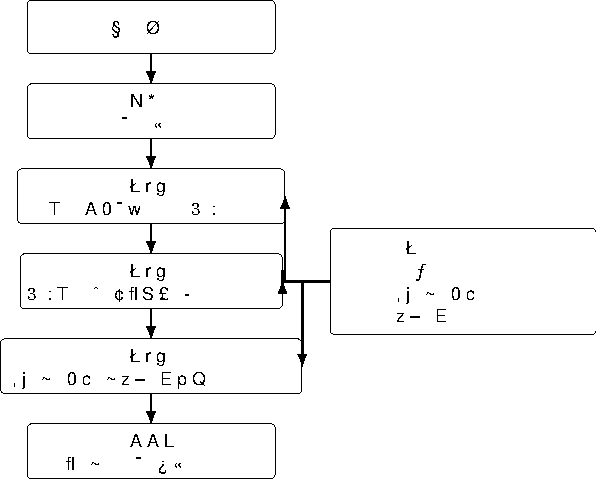
\includegraphics[width=0.94\columnwidth]{figure1.pdf}
\caption{想定するシステム構成．種目ごとの設定を共通処理に入力し，設定で対応できない場合は個別の処理を追加する．}
\label{fig:system}
\end{figure}

カメラ映像から姿勢推定を行い，ランドマークを取得する．その後，種目ごとの設定を使って評価に使用する3点を選び，角度を計算する．計算した角度を目標角度，許容範囲，比較条件と比べて，フォームの判定結果を出力する．このように，種目が変わっても同じ流れで処理できる部分を共通化する．

設定データには，(a)角度計算に使う3点のランドマーク名，(b)目標角度，(c)許容範囲，(d)比較条件を記述する．例えばスクワットでは「股関節・膝・足首」を指定し，膝角度90度，許容範囲$\pm15$度のように設定する．アームカールでは3点を「肩・肘・手首」に変更することで，同じ角度計算や判定処理を使えるようにする．

本研究で重要なのは，JSONという形式そのものではなく，設定だけで対応できる部分と，プログラムを追加する必要がある部分を分けることである．例えば，膝と股関節など複数の角度を同時に使う場合や，角度の変化，動作の順番などを使う場合は，現在の設定だけでは対応できない可能性がある．その場合は，共通の処理を追加するか，種目ごとの処理を追加する．このように，どこまで設定の変更だけで対応できるかを調べる．


\section{実装}

実装にはPython，OpenCV，MediaPipeを用いる．OpenCVはカメラ映像の取得や画像処理，MediaPipe Pose Landmarkerは人体のランドマークの取得に利用する[4,5]．姿勢推定によって取得したランドマークを使い，指定した3点から関節角度を計算する．

現在はスクワットを対象とした試作を行っており，Webカメラ映像の取得，姿勢推定，ランドマーク・骨格の表示，3点からの膝角度の計算，基準値との比較・判定，結果の表示，JSONからの設定値の読み込みまでを確認している．これにより，カメラ映像から姿勢を取得し，角度を計算して判定結果を表示する基本的な流れは確認できている．

ただし，現時点では共通化が完成したわけではなく，共通化に使う基本的な機能を確認している段階である．現在のコードでは，角度計算に使う股関節・膝・足首がコード内に固定されているため，設定を変更するだけで対象の関節を切り替えることはまだできていない．

また，設定ファイルの場所や，判定に必要な\texttt{tolerance}などの項目も整理する必要がある．今後は，角度計算に使う3点を設定ファイルから読み込み，スクワットとアームカールで同じ処理を使えるようにする．そのため，現在できている処理と，これから作る共通化の部分を分けて考える．


\section{検証方法と考察の観点}

まず，3章で考えた設定形式と共通処理を実装する．その上で，スクワットとアームカールの設定を用意し，同じプログラムで両方の種目を扱えるか確認する．また，計算した角度が正しいか，設定した条件に対して正しく判定できるかも確認する．

次に，評価方法を少しずつ変えて，どこまで設定だけで対応できるかを調べる．対象とするのは，(i)関節の指定だけが違う場合，(ii)複数の角度や条件を組み合わせる場合，(iii)角度の変化や動作の順番など，時間による変化を使う場合である．それぞれについて，設定だけで対応できるのか，共通のプログラムを追加する必要があるのか，それとも種目ごとのプログラムが必要なのかを確認する．

\begin{table}[t]
\centering
\caption{検証する評価方法と想定する対応}
\small
\begin{tabular}{p{0.29\columnwidth}p{0.23\columnwidth}p{0.39\columnwidth}}
\toprule
評価方法 & 主な違い & 確認する内容\\
\midrule
関節角度 & 対象3点 & 設定だけで変更できるか\\
複数条件 & 複数角度 & 共通処理で対応できるか\\
時間的変化 & フレーム間の関係 & 個別処理が必要か\\
\bottomrule
\end{tabular}
\end{table}

例えば，スクワットの膝角度とアームカールの肘角度では，使用する3点は異なるが，「3点から角度を計算して基準値と比べる」という処理は同じである．この場合に設定を変えるだけで動作すれば，関節の指定を設定に分ける方法が使えることを確認できる．

一方，膝角度と股関節角度を同時に判定する場合は，複数の角度を扱う処理が必要になる．また，立った状態から下降し，底まで下がってから立ち上がるといった動作の順番を判定する場合は，複数のフレームの情報を使う必要がある．このような違いを比較して，どのような評価方法なら設定だけで対応できるかを調べる．

角度計算と判定の正しさについても確認する．例えば，3点の位置関係から90度になる姿勢を用意し，システムが90度付近の値を出力するかを確認する．さらに，目標90度，許容範囲$\pm15$度と設定し，75度，90度，105度などの値を使って，判定結果が設定どおりになるかを確認する．

また，種目を追加したときのプログラムの変更量についても確認する．種目ごとに個別のプログラムを作った場合と比較し，どの部分を変更したか，どの程度のコードを追加したかを記録する．これによって，設定に分けることで実際にプログラムの修正を減らせるかを確認する．

なお，角度が設定した範囲に入ったことは，あくまで設定した基準に対する判定であり，それだけで「正しいフォーム」と判断するものではない．


\section{考察の観点}

検証した結果から，設定を変更するだけで対応できた評価方法と，プログラムの変更が必要だった評価方法を整理する．特に，関節の指定だけが異なる場合には設定だけで対応できるか，複数の条件や時間的な変化を扱う場合にはどのような追加処理が必要になるかを確認する．

設定だけでは対応できなかった場合には，どのような機能を追加すれば共通の処理として使えるのか，または種目ごとの処理にした方がよいのかを考える．例えば，複数の角度を設定できるようにすることで共通処理として対応できる場合もある．一方で，動作の順番など複雑な処理まで設定に入れると，設定ファイル自体が分かりにくくなる可能性がある．

そのため，設定に入れる部分と，プログラムとして分ける部分をどのように決めるかについて考察する．また，設定項目を増やすことで対応できる評価方法が増える一方で，設定が複雑になる可能性もあるため，どこまでを設定で扱うかについても検討する．

さらに，種目を追加したときに，実際にどの部分のプログラムを変更したかも確認する．これによって，共通化したことで既存のプログラムへの変更をどの程度減らせたかを確認する．


\section{おわりに}

本研究では，カメラ映像から姿勢を推定してフォームを評価するシステムを複数の種目に対応させる際の，プログラムの修正や保守の負担に着目した．そして，種目ごとに異なる部分を設定にまとめ，それ以外の処理を共通化する構成を考えた．

現在はスクワットの試作を行い，映像取得，姿勢推定，角度計算，判定，結果表示，JSONの読み込みまでを確認している．今後は設定ファイルとプログラムを整理し，角度計算に使う関節を設定から変更できるようにする．その上で，スクワットとアームカールを同じ処理で扱えるかを確認する．

その後，評価方法を変えながら検証し，設定だけで対応できる範囲と，プログラムの変更が必要になる範囲を明らかにする．また，種目を追加したときの変更量も確認し，今回考えた構成によってプログラムの修正をどの程度減らせるかを調べる．


\begin{thebibliography}{9}
\small
\setlength{\itemsep}{0pt}

\bibitem{tanabe}
田邉英介，椋木雅之，高塚佳代子：
運動過程をフィードバックする筋力トレーニング支援システム，
2021年度電気・情報関係学会九州支部連合大会講演論文集，
p.228，2021．

\bibitem{merca}
C. Mercadal-Baudart, C. Liu, G. Farrell, M. Boyne,
J. González Escribano, A. Smolic, C. Simms:
Exercise quantification from single camera view markerless 3D pose estimation,
Heliyon, Vol.10, No.6, e27596, 2024.

\bibitem{patidar}
K. Patidar, M. A. Zaveri:
Framework for Gym Posture Estimation Using MediaPipe and OpenCV,
2025 IEEE International Conference on Recent Advances in Computing and Systems (REACS),
DOI: 10.1109/REACS67479.2025.11413297, 2025.

\bibitem{mediapipe}
Google AI Edge: MediaPipe Pose Landmarker,
\url{https://ai.google.dev/edge/mediapipe/solutions/vision/pose_landmarker}
（参照 2026-09-21）．

\bibitem{opencv}
OpenCV: OpenCV Documentation,
\url{https://docs.opencv.org/4.x/}
（参照 2026-09-21）．

\end{thebibliography}

\end{document}
```
